\textit{Recommended reading:} FP Section 2.2 and 2.3 covers the basic deterministic inventory models that will be considered here. We suggest you to be familiar with that material. 


\begin{question}
The demand is never known in advance. If so, what is the use of a deterministic inventory models?
\end{question}

\begin{solution}
Indeed almost all inventory management environments demand is not known in advance. But there are many cases where the variability of the demand is so low that the uncertainty can be ignored. Also, it is not uncommon to have ``advance demand information'' in some industries where customers place their order before they actually want it to be delivered. If this is the case, then one can safely assume that the demand is known with certainty over some interval of time. 

From a theoretical point of view, these models can be used as points of reference while helping you to better understanding certain trade-offs. The EOQ model has very restrictive assumptions with respect to demand, yet it is one of the most well-known models by both academics and practitioners. Finally, deterministic models -- to a certain extent -- can be adapted to account for stochastic demands and used as heuristic approaches. We will see many examples of this in this course.  
\end{solution}

\begin{question}
The assumption of deterministic demands sounds like simplifying assumption in modeling inventories. What are it's implications?
\end{question}

\begin{solution}
Obviously knowing the demand make an inventory manager's life much easier. The main implication is simple: when you take an action, say place a replenishment order, you know exactly how this will effect the system in the future. Probably the most important result of this is that the optimal answers to the fundamental inventory control questions will not change over time as a response to realized demands. 
\end{solution}

\subsection{EOQ and Extensions}

The most well-known deterministic inventory model is the EOQ model. In the following exercises we are going to modify the assumptions of the EOQ model with the aim to investigate how the environment affects the inventory model. Before proceeding further, have another look at Exercise~\ref{ex:1} and recap the assumptions of the EOQ model.

\begin{question}
Explain the inventory policy behind the EOQ model. What are its parameters? How does it work?
\end{question}

  \begin{solution}
It is a very simple policy. It has a single parameter $Q$. It works as follows: place an order of size $Q$ whenever the inventory level hits the level 0.
  \end{solution}
  
\begin{question}
For the sake of comparison, sketch how the inventory behaves over time for the EOQ model. Then write down the cost function and characterize the optimal order quantity.
\end{question}

\begin{solution}
See Figure~\ref{fig:EOQ}.

\begin{figure}[htbp]
\centering
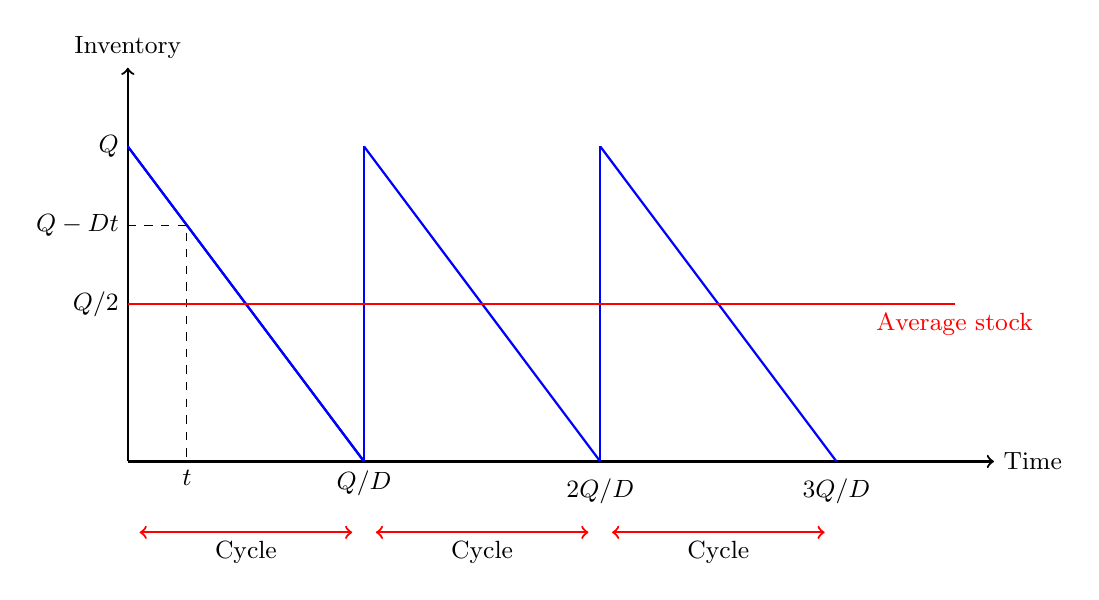
\begin{tikzpicture}[x=1cm,y=0.02cm]
\small
\draw[thick,->] (0,0) -- (11,0) node[right] {Time};
\draw[thick,->] (0,0) -- (0,250) node[above] {Inventory};
\draw[] (0,200) node[left] {$Q$};
\draw[color=blue,thick] (0,200) -- (3,0);
\draw[] (0.75,0) node[below] {$t$};
\draw[] (0,150) node[left] {$Q-Dt$};
\draw[dashed] (0,150) -- (0.75,150) -- (0.75,0);
\draw[] (3,0) node[below] {$Q / D$};
\foreach \y in {1,...,3}{
	\draw[color=blue,thick] (3*\y-3,200) -- (3*\y,0);}
\foreach \y in {1,2}{
	\draw[color=blue,thick] (3*\y,0) -- (3*\y,200);}
\foreach \y in {2,3}{
	\draw[] (3*\y,-5) node[below] {\y $Q/D$};}
\draw[] (0,100) node[left] {$Q / 2$};
\draw[color=red,thick] (0,100) -- (10.5,100) node[below] {Average stock};
\foreach \y in {0,...,2}{
	\draw[color=red,thick,<->] (3*\y+0.15,-45) -- (3*\y+3-0.15,-45);
	\draw[] (3*\y+1.5,-45) node[below] {Cycle};}
\end{tikzpicture}
\caption{EOQ model}
\label{fig:EOQ}
\end{figure}


The total cost for one cycle is the sum of ordering cost, procurement cost, and inventory (holding) cost. The order cost is $A$ per cycle as we order only once in each cycle. The procurement cost equals the unit procurement cost times the order quantity $cQ$, i.e. we buy just enough to satisfy all the demand in each cycle. The inventory cost per cycle is the total area of the triangle times $h$, i.e. 
\begin{equation*}
h~\frac{\text{height}\cdot\text{base}}{2} = h~\frac{Q \cdot Q/D }{2} = \frac{hQ^2}{2D}.
\end{equation*}

Thus, the total cycle cost is $A+cQ+\frac{hQ^2}{2D}$. The average cost per unit time is this total cost divided by the duration of one cycle, which is $\frac{Q}{D}$. Therefore, the average cost is
\begin{equation*}
A \frac{D}{Q}+cQ \frac{D}{Q} + \frac{hQ^2}{2D} \frac{D}{Q} = \frac{AD}{Q}+cD+\frac{hQ}{2}
\end{equation*}

This expression gives us the average cost as a function of the order quantity:
\begin{equation*}
f(Q) = \frac{AD}{Q}+cD+\frac{hQ}{2}.
\end{equation*}

The average cost function $f(Q)$ is differentiable and convex and therefore one can easily compute the optimal order quantity  (we omit the proof as it immediately follows the first and second-order necessary conditions of optimality) by means of the EOQ formula
\begin{align*}
Q^*=\sqrt{\frac{2AD}{h}}.
\end{align*}

Then, the cost per unit time if we use the optimal order quantity can be written as 
\begin{equation*}
f(Q^*) = \frac{AD}{\sqrt{\frac{2AD}{h}}}+cD+\frac{h\sqrt{\frac{2AD}{h}}}{2} = \sqrt{2ADh} + cD
\end{equation*}


\end{solution}

\begin{question}
To better understand how the cost function looks like, sketch the cost function as well as its three components. Do this with different cost parameters and see how they affect the resulting figure as well as the optimal order quantity.
\end{question}

\begin{solution}
See Figure~\ref{fig:EOQ_effects}.

\begin{figure}[htbp]
\begin{subfigure}[b]{0.5\textwidth}
\begin{center}
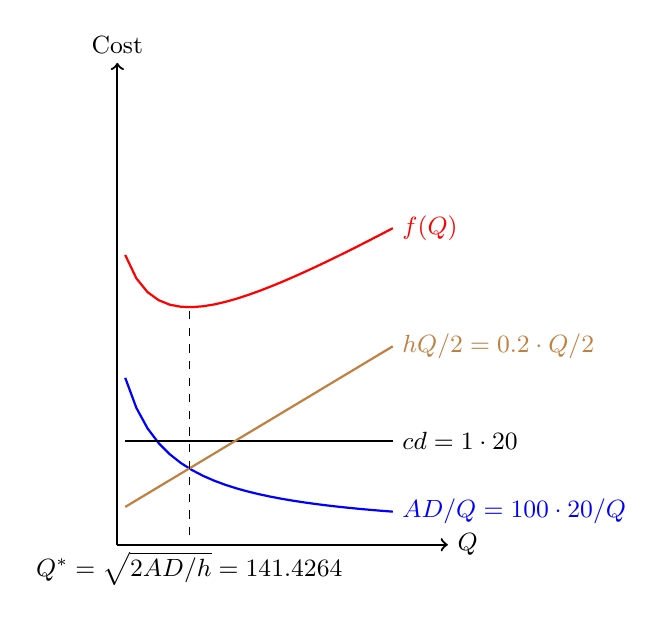
\begin{tikzpicture}[x=0.01cm,y=0.06cm]
\small
\def\c{1} 
\def\K{100} 
\def\h{0.2} 
\def\d{20} 
\pgfmathsetmacro{\Q}{sqrt(2)*sqrt(\K)*sqrt(\d)/sqrt(\h)}
\pgfmathsetmacro{\f}{sqrt(2)*sqrt(\K)*sqrt(\d)*sqrt(\h)+\c*\d}	
\draw[thick,->] (50,-2) -- (470,-2) node[right] {$Q$};
\draw[thick,->] (50,-2) -- (50,100) node[above] {Cost};
\draw[color=blue,thick,domain=60:400] plot (\x,{\d*\K/\x}) node[right] {$AD / Q = \K\cdot\d / Q$};
\draw[color=black,thick,domain=60:400] plot (\x,{\c*\d}) node[right] {$cd = \c\cdot \d$};
\draw[color=brown,thick,domain=60:400] plot (\x,{\h*\x/2}) node[right] {$hQ / 2 = \h\cdot Q / 2$};
\draw[color=red,thick,domain=60:400] plot (\x,{\d*\K/\x+\c*\d+\h*\x/2}) node[right] {$f(Q)$};
\draw (\Q,-1.5) node[below] {$Q^{*} = \sqrt{2AD / h} = \Q$};
\draw[dashed] (\Q,0) -- (\Q,\f);
\end{tikzpicture}
\end{center}
\caption{$A=100$ $c=1$ $h=0.2$ $D=20$}
\label{fig:eoq1}
\end{subfigure}
~
\begin{subfigure}[b]{0.5\textwidth}
\begin{center}
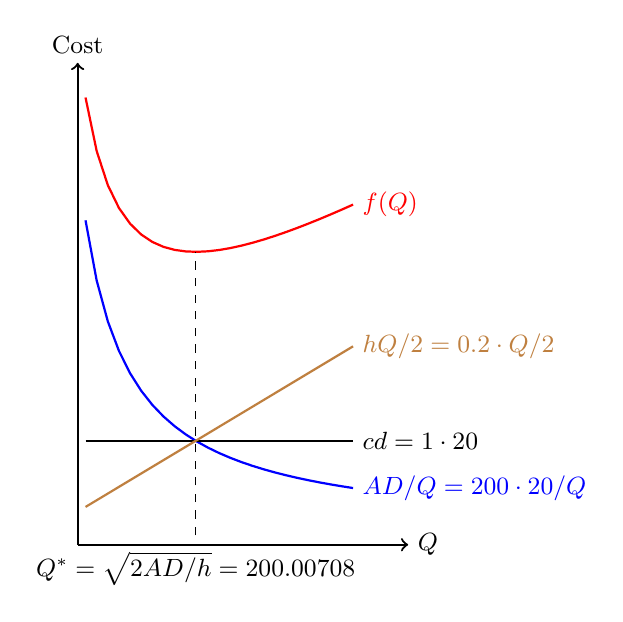
\begin{tikzpicture}[x=0.01cm,y=0.06cm]
\small
\def\c{1} 
\def\K{200} 
\def\h{0.2} 
\def\d{20} 
\pgfmathsetmacro{\Q}{sqrt(2)*sqrt(\K)*sqrt(\d)/sqrt(\h)}
\pgfmathsetmacro{\f}{sqrt(2)*sqrt(\K)*sqrt(\d)*sqrt(\h)+\c*\d}	
\draw[thick,->] (50,-2) -- (470,-2) node[right] {$Q$};
\draw[thick,->] (50,-2) -- (50,100) node[above] {Cost};
\draw[color=blue,thick,domain=60:400] plot (\x,{\d*\K/\x}) node[right] {$AD / Q = \K\cdot\d / Q$};
\draw[color=black,thick,domain=60:400] plot (\x,{\c*\d}) node[right] {$cd = \c\cdot \d$};
\draw[color=brown,thick,domain=60:400] plot (\x,{\h*\x/2}) node[right] {$hQ / 2 = \h\cdot Q / 2$};
\draw[color=red,thick,domain=60:400] plot (\x,{\d*\K/\x+\c*\d+\h*\x/2}) node[right] {$f(Q)$};
\draw (\Q,-1.5) node[below] {$Q^{*} = \sqrt{2AD / h} = \Q$};
\draw[dashed] (\Q,0) -- (\Q,\f);
\end{tikzpicture}
\end{center}
\caption{$A=200$ $c=1$ $h=0.2$ $D=20$}
\label{fig:eoq2}
\end{subfigure}
\\
\begin{subfigure}[b]{0.5\textwidth}
\begin{center}
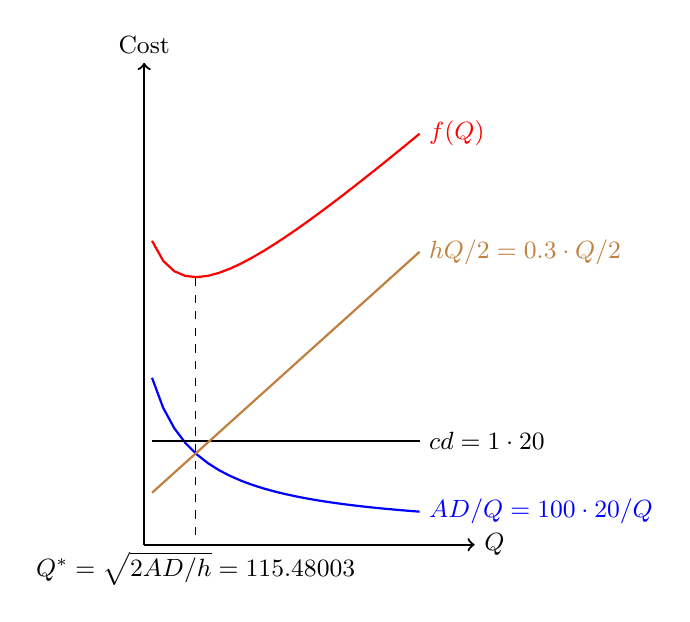
\begin{tikzpicture}[x=0.01cm,y=0.06cm]
\small
\def\c{1} 
\def\K{100} 
\def\h{0.3} 
\def\d{20} 
\pgfmathsetmacro{\Q}{sqrt(2)*sqrt(\K)*sqrt(\d)/sqrt(\h)}
\pgfmathsetmacro{\f}{sqrt(2)*sqrt(\K)*sqrt(\d)*sqrt(\h)+\c*\d}	
\draw[thick,->] (50,-2) -- (470,-2) node[right] {$Q$};
\draw[thick,->] (50,-2) -- (50,100) node[above] {Cost};
\draw[color=blue,thick,domain=60:400] plot (\x,{\d*\K/\x}) node[right] {$AD / Q = \K\cdot\d / Q$};
\draw[color=black,thick,domain=60:400] plot (\x,{\c*\d}) node[right] {$cd = \c\cdot \d$};
\draw[color=brown,thick,domain=60:400] plot (\x,{\h*\x/2}) node[right] {$hQ / 2 = \h\cdot Q / 2$};
\draw[color=red,thick,domain=60:400] plot (\x,{\d*\K/\x+\c*\d+\h*\x/2}) node[right] {$f(Q)$};
\draw (\Q,-1.5) node[below] {$Q^{*} = \sqrt{2AD / h} = \Q$};
\draw[dashed] (\Q,0) -- (\Q,\f);
\end{tikzpicture}
\end{center}
\caption{$A=200$ $c=1$ $h=0.3$ $D=20$}
\label{fig:eoq3}
\end{subfigure}
~
\begin{subfigure}[b]{0.5\textwidth}
\begin{center}
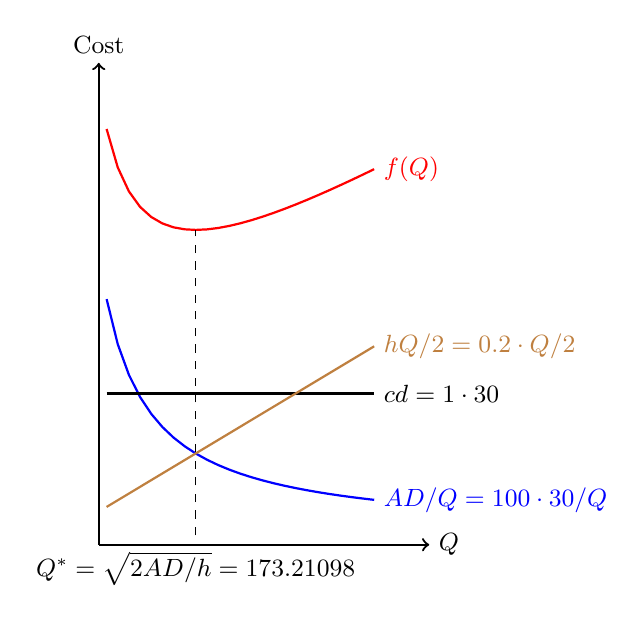
\begin{tikzpicture}[x=0.01cm,y=0.06cm]
\small
\def\c{1} 
\def\K{100} 
\def\h{0.2} 
\def\d{30} 
\pgfmathsetmacro{\Q}{sqrt(2)*sqrt(\K)*sqrt(\d)/sqrt(\h)}
\pgfmathsetmacro{\f}{sqrt(2)*sqrt(\K)*sqrt(\d)*sqrt(\h)+\c*\d}	
\draw[thick,->] (50,-2) -- (470,-2) node[right] {$Q$};
\draw[thick,->] (50,-2) -- (50,100) node[above] {Cost};
\draw[color=blue,thick,domain=60:400] plot (\x,{\d*\K/\x}) node[right] {$AD / Q = \K\cdot\d / Q$};
\draw[color=black,thick,domain=60:400] plot (\x,{\c*\d}) node[right] {$cd = \c\cdot \d$};
\draw[color=brown,thick,domain=60:400] plot (\x,{\h*\x/2}) node[right] {$hQ / 2 = \h\cdot Q / 2$};
\draw[color=red,thick,domain=60:400] plot (\x,{\d*\K/\x+\c*\d+\h*\x/2}) node[right] {$f(Q)$};
\draw (\Q,-1.5) node[below] {$Q^{*} = \sqrt{2AD / h} = \Q$};
\draw[dashed] (\Q,0) -- (\Q,\f);
\end{tikzpicture}
\end{center}
\caption{$A=100$ $c=1$ $h=0.2$ $D=30$}
\label{fig:eoq4}
\end{subfigure}
\caption{Effects of different parameter values}
\label{fig:EOQ_effects}
\end{figure}

\end{solution}

\begin{question}
The EOQ formula suggests that the optimal order quantity is independent of the unit procurement cost. Does it make sense?
\end{question}

\begin{solution}
Yes. We know that the procurement cost per cycle is $cQ$ and the average procurement cost per unit time is $cQ\frac{D}{Q}=cD$. This is actually obvious. Because we satisfy all demand, we procure for all demand. Therefore, on the long term what we buy equals the demand; and as the procurement cost is the same over time, the average procurement cost per unit time should indeed be $cD$. Because it is a constant that is independent of $Q$, it has no effect on the optimal order quantity.
\end{solution}

\begin{question}
All the figures suggest that the optimal order quantity is such an order quantity where the ordering and inventory costs per unit time are the same. Is it always the case?
\end{question}

\begin{solution}
Yes. A formal proof can also be provided, but the intuition behind it is more important and it is rather simple. Because average procurement cost per unit time is constant, the cost trade-off lies in ordering and inventory costs per unit time. It is easy to see that the average ordering cost is decreasing in $Q$ and the average holding cost is increasing in $Q$ (see formulas and figures). Therefore, it is always better to choose a $Q$ such that these cost are balanced.
\end{solution}

\begin{question}
  It is very important to know that the total inventory cost for
  the EOQ model is quite insensitive to the actual order quantity
  $Q$. Show this for the case with $A=100$, $h=0.2$, $c=1$, and $D=20$. What
  happens to the total cost if $Q=60, 80, \ldots 200$?
\end{question}

  \begin{solution}

If we plug in the parameters we obtain from the EOQ formula that $Q^{*} \approx 141.42$ units and $f(Q^{*}) \approx \mathdollar 48.28$.

See Table~\ref{tab:sensitivity}
\begin{table}[htbp]
  \centering
    \begin{tabular}{rrrrr}
    \toprule
    $Q$   & $AD/Q$  & $cD$  & $hQ/2$  & $f(Q)$ \\
    \midrule
    60    & 33.33   & 20.00 & 6.00    & 59.33 \\
    80    & 25.00   & 20.00 & 8.00    & 53.00 \\
    100   & 20.00   & 20.00 & 10.00   & 50.00 \\
    120   & 16.67   & 20.00 & 12.00   & 48.67 \\
    140   & 14.29   & 20.00 & 14.00   & 48.29 \\
    160   & 12.50   & 20.00 & 16.00   & 48.50 \\
    180   & 11.11   & 20.00 & 18.00   & 49.11 \\
    200   & 10.00   & 20.00 & 20.00   & 50.00 \\
    \bottomrule
    \end{tabular}%
\caption{Sensitivity of the EOQ}
\label{tab:sensitivity}
\end{table}%
  \end{solution}

\begin{question}
  As a first variation, what would you change/do if the lead time
  is no longer 0, but a positive constant  $L$? Thus, all the other
  assumptions of the EOQ model stay the same, only the lead time
  becomes positive.  In other words, how would you change the EOQ
  policy, and determine when and how to order?

\end{question}

  \begin{solution}
    The answer is simple. Because stock-outs are not allowed, we order early. See Figure~\ref{fig:EOQleadtime}.

\begin{figure}[htbp]
\centering
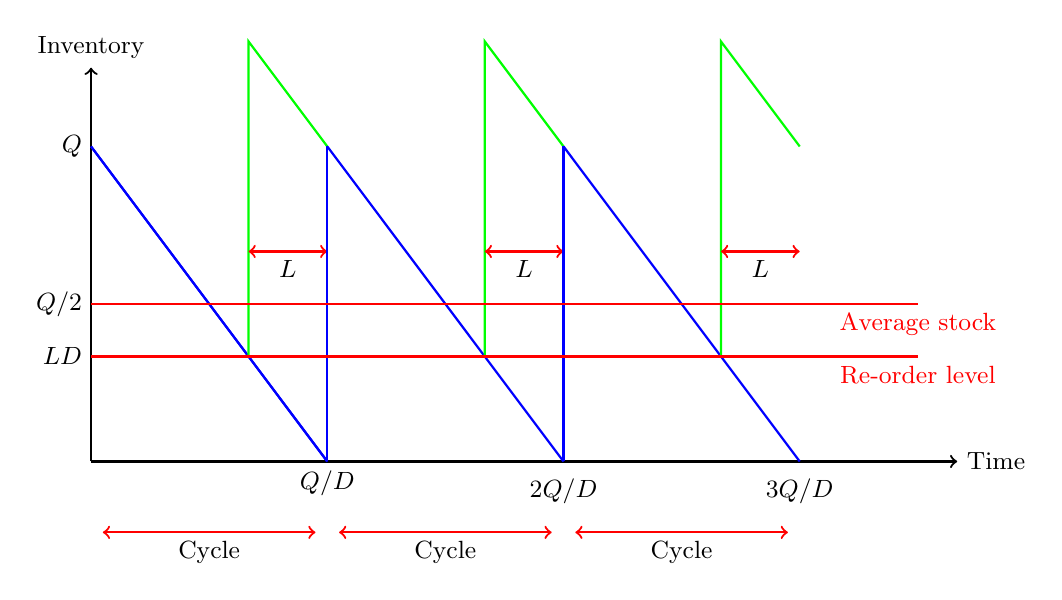
\begin{tikzpicture}[x=1cm,y=0.02cm]
\small
\draw[thick,->] (0,0) -- (11,0) node[right] {Time};
\draw[thick,->] (0,0) -- (0,250) node[above] {Inventory};
\draw[] (0,200) -- (0,200) node[left] {$Q$};
\draw[color=blue,thick] (0,200) -- (3,0);
\draw[] (3,0) node[below] {$Q / D$};
\foreach \y in {1,...,3}{
	\draw[color=blue,thick] (3*\y-3,200) -- (3*\y,0);
	\draw[color=green,thick] (3*\y-3+2,200/3) -- (3*\y-3+2,200/3*4) -- (3*\y,200);
	\draw[color=red,thick,<->] (3*\y-3+2,200/3*2) -- (3*\y,200/3*2);
	\draw[] (3*\y-3+2.5,200/3*2) node[below] {$L$};}
\foreach \y in {1,2}{
	\draw[color=blue,thick] (3*\y,0) -- (3*\y,200);}
\foreach \y in {2,3}{
	\draw[] (3*\y,-5) node[below] {\y $Q/D$};}
\draw[] (0,100) node[left] {$Q / 2$};
\draw[color=red,thick] (0,100) -- (10.5,100) node[below] {Average stock};
\draw[] (0,200/3) node[left] {$L D$};
\draw[color=red,thick] (0,200/3) -- (10.5,200/3) node[below] {Re-order level};
\foreach \y in {0,...,2}{
	\draw[color=red,thick,<->] (3*\y+0.15,-45) -- (3*\y+3-0.15,-45);
	\draw[] (3*\y+1.5,-45) -- (3*\y+1.5,-45) node[below] {Cycle};}
\end{tikzpicture}
\caption{EOQ model with lead times}
\label{fig:EOQleadtime}
\end{figure}

    
This new policy can be described in a simple way by introducing the
concept of \emph{inventory position}, that is, all stock on-hand plus
the replenishments under way. The green graph above illustrates the
inventory position $IP$. When $IP$ hits the lead time demand $L D$,
i.e., the lead time $L$ times the demand $D$, we should order
$Q$. During the lead time $L$ the demand will be met from on-hand
stock. When the replenishment arrives a lead time $L$ later, it
arrives just in time to meet the demand again.

The cost analysis remains unchanged, as the effect of the lead time is solely on the point in time where a replenishment order is placed, and not on the frequency of orders and/or the actual stock levels. 
  \end{solution}

\begin{question}
Explain how the inventory policy can be described in presence of a positive lead time. What are its parameters? How does it work?
\end{question}

  \begin{solution}
It is still a very simple policy. It has a single parameter $Q$. It works as follows: place an order of size $Q$ whenever the inventory level hits the level $LD$.
  \end{solution}



\begin{question}
  What would happen stock-outs were allowed and demand during stock-outs were backordered? Let's first assume that the backordering cost is $b$ per unit per time. That is, for each customer we pay $b$ per unit time.  As we know already know the effect of positive lead times, we will assume that the lead time is zero.
  
Sketch how the inventory behaves over time for the EOQ model with backorders. Then write down the cost function and characterize the optimal order quantity and backorder level.
\end{question}

\begin{solution}
The dynamics of the new system are illustrated in Figure~\ref{fig:EOQ_backorders}. 

\begin{figure}[htbp]
\centering
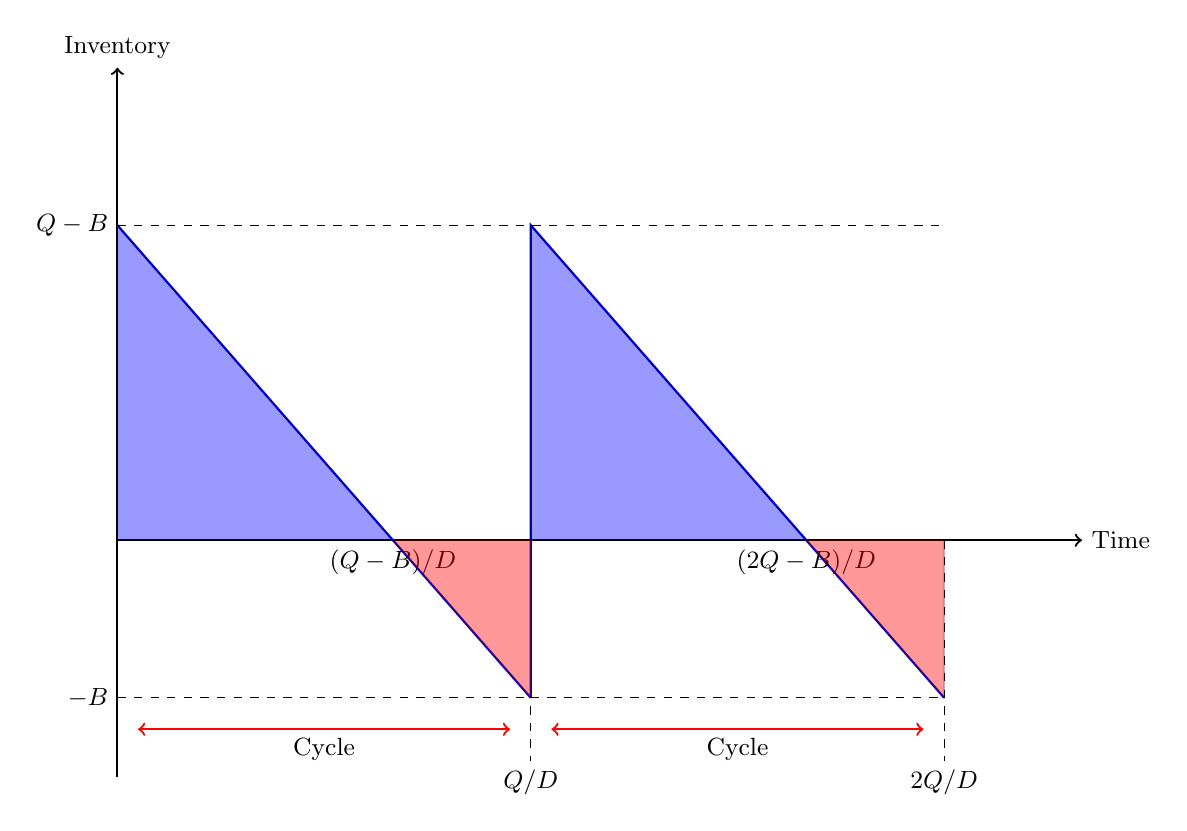
\begin{tikzpicture}[x=1.75cm,y=0.02cm]
\small
\draw[thick,->] (0,0) -- (7,0) node[right] {Time};
\draw[thick,->] (0,-150) -- (0,300) node[above] {Inventory};
\draw[] (0,200) node[left] {$Q - B$};
\draw[color=blue,thick] (0,200) -- (3,-100);
\draw[] (0,-100) node[left] {$-B$};
\draw[dashed] (0,-100) -- (3,-100);
\draw[] (2,0) node[below] {$(Q - B) / D$};
\draw[dashed] (3,0) -- (3,-140) node[below] {$Q / D$};
\draw[color=blue,thick] (3,-100) -- (3,200) -- (6,-100);
\draw[] (5,0) node[below] {$(2Q - B) / D$};
\draw[dashed] (6,0) -- (6,-140) node[below] {$2Q / D$};
\draw[dashed] (0,200) -- (6,200);
\draw[dashed] (3,-100) -- (6,-100);
\draw [fill=blue,opacity=.4] (0,0) -- (0,200) -- (2,0) -- cycle;
\draw [fill=blue,opacity=.4] (3,0) -- (3,200) -- (5,0) -- cycle;
\draw [fill=red,opacity=.4] (2,0) -- (3,-100) -- (3,0) -- cycle;
\draw [fill=red,opacity=.4] (5,0) -- (6,-100) -- (6,0) -- cycle;
\foreach \y in {0,1}{
	\draw[color=red,thick,<->] (3*\y+0.15,-120) -- (3*\y+3-0.15,-120);
	\draw[] (3*\y+1.5,-120) node[below] {Cycle};}
\end{tikzpicture}  
\caption{EOQ model with backorders}
\label{fig:EOQ_backorders}
\end{figure}


Here, we order $Q$ units every $\frac{Q}{D}$ time units. However, we replenishing inventories when the stock level hits some level $-B$, rather than zero. In each replenishment cycle of length $\frac{Q}{D}$; we spend $\frac{Q-B}{D}$ units of time while having inventories and $\frac{B}{D}$ units of time having stock-outs. 



The total cost for one cycle is the sum of ordering cost, procurement cost, and the inventory (holding and backorder) cost. The order cost is $A$ per cycle as we order only once in each cycle. The procurement cost equals the unit procurement cost times the order quantity $cQ$, i.e. we buy just enough to satisfy all the demand in each cycle. The holding cost per cycle is the total area of the blue triangle times $h$, i.e. 
\begin{equation*}
h~\frac{\text{height}\cdot\text{base}}{2} = h~\frac{(Q-B) \cdot (Q-B)/D}{2} = \frac{h(Q-B)^2}{2D}.
\end{equation*}

The backorder cost per cycle is the total area of the red triangle times $b$, i.e. 
\begin{equation*}
b~\frac{\text{height}\cdot\text{base}}{2} = b~\frac{B \cdot B/D}{2} = \frac{hB^2}{2D}.
\end{equation*}

Thus, the total cycle cost is $A+cQ+\frac{h(Q-B)^2}{2D}+\frac{hB^2}{2D}$. The average cost per unit time is this total cost divided by the duration of one cycle, which is $\frac{Q}{D}$. Therefore, the average cost is
\begin{equation*}
A \frac{D}{Q}+cQ \frac{D}{Q} + \frac{h(Q-B)^2}{2D} \frac{D}{Q} + \frac{hB^2}{2D} \frac{D}{Q} = \frac{AD}{Q}+cD+\frac{h(Q-B)^2}{2Q} + \frac{bB^2}{2Q}.
\end{equation*}

This expression gives us the average cost as a function of the order quantity and backorder level:
\begin{equation*}
f(Q,B) = \frac{AD}{Q}+cD+\frac{h(Q-B)^2}{2Q} + \frac{bB^2}{2Q}.
\end{equation*}

Notice that by setting $B=0$ we get the standard EOQ cost function.

The average cost function $f(Q,B)$ is differentiable and jointly convex. Therefore one can easily compute the optimal order quantity and backorder level (we omit the proof) by means of the following formulas.
\begin{align*}
Q^* = \sqrt{\frac{2AD}{h}} \sqrt{\frac{h+b}{b}} \\
B^* = Q^* \frac{h}{h+b} 
\end{align*}

Then, the cost per unit time if we use the optimal order quantity and backorder level can be written as 
\begin{align*}
f(Q^*,B^*) 
%& = \frac{AD}{\sqrt{\frac{2AD}{h}} \sqrt{\frac{h+b}{b}}}+cD+
%\frac{h\left(\sqrt{\frac{2AD}{h}} \sqrt{\frac{h+b}{b}}-\left(\sqrt{\frac{2AD}{h}} \sqrt{\frac{h+b}{b}}\right) \frac{h}{h+b}\right)^2}{2\sqrt{\frac{2AD}{h}} \sqrt{\frac{h+b}{b}}} + 
%\frac{b\left(\left(\sqrt{\frac{2AD}{h}} \sqrt{\frac{h+b}{b}}\right)\frac{h}{h+b}\right)^2}{2\sqrt{\frac{2AD}{h}} \sqrt{\frac{h+b}{b}}} \\
& = \sqrt{2ADh} \sqrt{\frac{b}{h+b}} + cD
\end{align*}
\end{solution}


\begin{question}
What happens to the optimal order quantity $Q^*$, backorder level $B^*$, and optimal average cost per unit time in response to different backorder costs? 

Show these for the case with $A=100$, $h=0.2$, $c=1$, and $D=20$. What
  happens if $b=0.5,1.0,\ldots 10.0$?

\end{question}

\begin{solution}
Let's explain based on the following interesting observations: 
\begin{enumerate}
\item The formula for the optimal order quantity is a slight modification of the formula derived for the no-stock-out case. We simply multiply it with the constant $\sqrt{\frac{h+b}{b}}$. If $b$ is extremely large, then this constant approaches 1 and we have the same optimal order quantity with the no-stock-out case. 

For arbitrary values of $b$ the constant will be larger than 1. Therefore, we can conclude that the optimal order quantity will be higher as compared to the no-stock-out case and the difference will be larger for smaller values of $b$. 

\item The optimal backorder level is a constant fraction of the order quantity. This fraction $\frac{h}{h+b}$ in fact reflects on the trade-off between the holding and backorder costs. For instance, if $b=9h$, then the backorder level should be 10\% of the order quantity. Furthermore, this immediately means that you should spend 10\% of the time with stock-outs and the remaining 90\% with inventories. 

If we put together this with our previous observation; we can conclude that a small backorder cost leads to (1) large order quantities, and (2) backorder levels being even larger fractions of the order quantities. 

\item The optimal average cost can also be obtained with a slight modification of the original one. The procurement costs remain the same but we simply multiply the inventory costs with the constant $\sqrt{\frac{b}{h+b}}$. If $b$ is extremely large, then this constant approaches 1 and we have the same optimal cost with the no-stock-out case. 

For arbitrary values of $b$ the constant will be smaller than 1. Therefore, we can conclude that the optimal average cost will be higher as compared to the no-stock-out case and the difference will be larger for smaller values of $b$. 
\end{enumerate}

Let's numerically analyze these effects. We know for the no-stockout case that if we plug in the parameters we obtain from the EOQ formula that $Q^{*} \approx 141.42$ units and $f(Q^{*}) \approx \mathdollar 48.28$. For different values of $b$ we obtain the results in Table~\ref{tab:effect_backorder}. 

\begin{table}[h]
  \centering
    \begin{tabular}{rrrr}
    \toprule
    $b$ & $Q^*$ & $B^*$ & $f(Q^*,B^*)$ \\
    \midrule
    0.5   & 167.33 & 47.81 & 43.90 \\
    1.0   & 154.92 & 25.82 & 45.82 \\
    1.5   & 150.55 & 17.71 & 46.57 \\
    2.0   & 148.32 & 13.48 & 46.97 \\
    2.5   & 146.97 & 10.89 & 47.22 \\
    3.0   & 146.06 & 9.13  & 47.39 \\
    3.5   & 145.41 & 7.86  & 47.51 \\
    4.0   & 144.91 & 6.90  & 47.60 \\
    4.5   & 144.53 & 6.15  & 47.68 \\
    5.0   & 144.22 & 5.55  & 47.74 \\
    5.5   & 143.97 & 5.05  & 47.78 \\
    6.0   & 143.76 & 4.64  & 47.82 \\
    6.5   & 143.58 & 4.29  & 47.86 \\
    7.0   & 143.43 & 3.98  & 47.89 \\
    7.5   & 143.29 & 3.72  & 47.91 \\
    8.0   & 143.18 & 3.49  & 47.94 \\
    8.5   & 143.08 & 3.29  & 47.96 \\
    9.0   & 142.98 & 3.11  & 47.98 \\
    9.5   & 142.90 & 2.95  & 47.99 \\
    10.0  & 142.83 & 2.80  & 48.01 \\
	1000.0	& 141.44 & 0.03	& 48.28 \\
    \bottomrule
    \end{tabular}%
   \caption{The effect of backorder cost}
  \label{tab:effect_backorder}%
\end{table}%

Note that all numbers are in line with our expectations. For instance, for increasing values of backorder cost, $Q^*$ and $B^*$ both decrease and the optimal average cost increases. Notice that the last row stands for a 'very large' backorder cost. Here, we see that the optimal backorder level is almost zero, and the optimal order quantity and the optimal average cost are almost the same with no-stock-out case. 
\end{solution}


\begin{question}
Explain the inventory policy behind the EOQ model with backlogging. What are its parameters? How does it work?
\end{question}

  \begin{solution}
It is a simple policy. It has two parameters $Q$ and $B$. It works as follows: place an order of size $Q$ whenever the backorder level reaches $B$.
  \end{solution}


\begin{question}
  Let us consider once again the original EOQ model and imagine a situation where items or ordering
  costs are so high that it is better not to `enter the business' at
  all. Can you find a condition to decide whether to keep inventories
  and satisfy demand or reject all demand and have no inventories?
\end{question}

  \begin{solution}
  
	The EOQ model is based on the assumption that we indeed satisfy the demand in the long term. The reason behind this assumption is our initial idea that it is 'profitable' to stay in the game. We now challenge that initial idea. 
	
	To begin with, we need to introduce an incentive to stay in the game. For instance, a revenue from sales. Let's assume that our selling price for item is $p$. If we satisfy the demand in the long term, we know that our average revenue per unit time would be $pD$. Observe that it works exactly the same way with average procurement cost which was $cD$. The average revenue per unit time is independent of the order quantity. That is, we obtain this revenue regardless of which inventory policy we use. 
	
	Now let's turn back to the question of whether or not to staying in the game. If we stayed in the game and employed the optimal ordering policy; our average revenue would be $pD$ and our average total cost will be $f(Q^*)=\sqrt{2ADh}+cD$. This would lead to a net profit of $(p-c)D-\sqrt{2ADh}$. If this value is positive, or put in other words, if we make profit, then we would stay in the business. 
  \end{solution}


\begin{question}
In many practical environments, there is economies of scale in ordering due to quantity discounts. How would this affect the EOQ model?
\end{question}

\begin{solution}
In presence of quantity discounts, we have an incentive to order more since the unit procurement cost decreases with the order size. This can be conceptualized by re-writing procurement cost as a function of the order quantity. There is also an interesting point that relates to the holding costs. It is often assumed that the unit holding cost is a fraction of the unit procurement cost. For instance, the holding cost per year is 30\% of the procurement cost. In case of quantity discounts, this implies that the holding cost is also a function of the order quantity. 
\end{solution}

\begin{question}
What are the most common discounting schemes? How do they work?
\end{question}

\begin{solution}
There are two common discounting schemes: all-unit discounts and incremental discounts. We discuss them below by means of examples. 

To emphasize the differences between these schemes, we make use a total procurement cost function $c(Q)$, i.e. we pay $c(Q)$ in total if we buy $Q$ units. The shape of $c(Q)$ obviously depends on the discounting scheme.

\paragraph{All-unit discounts} In this example, we have all-unit discounting with three discount intervals; $[0,100)$ interval with price \$1, $[100,200)$ interval with price \$0.8, and $[200,\infty)$ interval with price \$0.6. The discount is applied to all units. For instance, if we buy 120 items, then we pay in total $120\cdot 0.8=\$96$. The total procurement cost function $c(Q)$ of this discounting scheme is illustrated in Figure~\ref{fig:allunit}.

\begin{figure}[htbp]
\centering
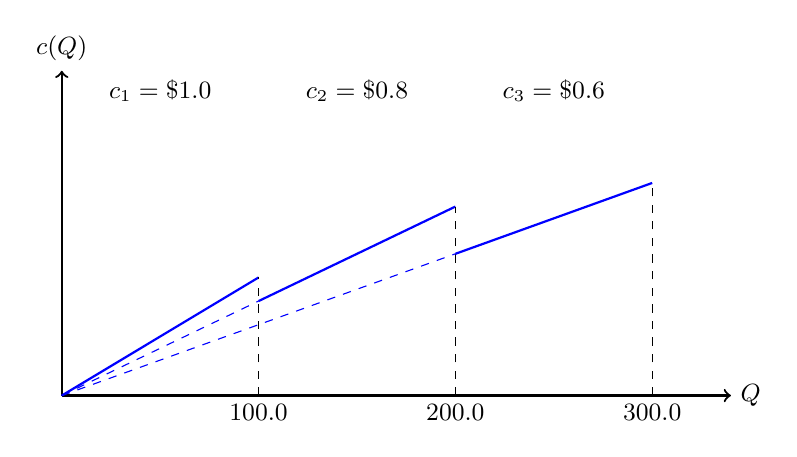
\begin{tikzpicture}[x=0.025cm,y=0.015cm]
\small
\draw[thick,->] (0,0) -- (340,0) node[right] {$Q$};
\draw[thick,->] (0,0) -- (0,275) node[above] {$c(Q)$};
\def\w{100}
\foreach \n/\a in {1/1.0,2/0.8,3/0.6}{
	\pgfmathsetmacro{\s}{(\n-1)*\w}	
	\pgfmathsetmacro{\e}{\n*\w}
	\draw[thick,color=blue,domain=\s:\e] plot (\x,{\a*\x});
	\draw[dashed,color=blue,domain=0:{\s+0.01}] plot (\x,{\a*\x});
	\draw[] (\e,0) -- (\e,0) node[below] {$\e$};
	\draw[dashed] (\e,0) -- (\e,\e*\a);
	\draw[] ({(\s+\e)/2},275) -- ({(\s+\e)/2},275) node[below] {$c_{\n} = \mathdollar\a$};}
\end{tikzpicture}
\caption{All-unit discounts}
\label{fig:allunit}
\end{figure}


\paragraph{Incremental discounts} In this example, we have incremental discounting with exactly the same discount intervals from the previous example. The difference here is that the discount is applied by parts. That is, we pay \$1 per unit for the part of the order that is below 100, we pay \$0.8 for the part of the order that is between 100 and 200, and we pay \$0.6 for the part of the order that is above 200. For instance, if we buy 120 items, then we pay in total $100\cdot 1 + 20 \cdot 0.8=116$. The total procurement cost function $c(Q)$ of this discounting scheme is illustrated in Figure~\ref{fig:incremental}.

\begin{figure}[htbp]
\centering
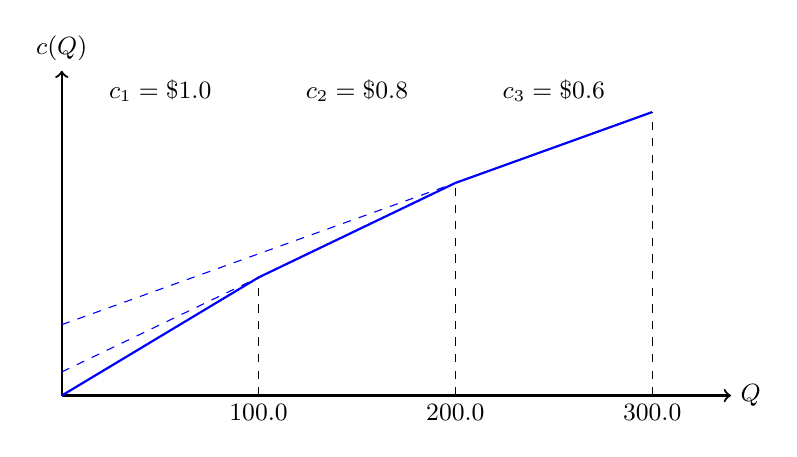
\begin{tikzpicture}[x=0.025cm,y=0.015cm]
\small
\draw[thick,->] (0,0) -- (340,0) node[right] {$Q$};
\draw[thick,->] (0,0) -- (0,275) node[above] {$c(Q)$};
\def\w{100}
\pgfmathsetmacro{\b}{0}
\foreach \n/\a/\b in {1/1.0/0,2/0.8/20,3/0.6/60}{
	\pgfmathsetmacro{\s}{(\n-1)*\w}	
	\pgfmathsetmacro{\e}{\n*\w}
	\draw[thick,color=blue,domain=\s:\e] plot (\x,{\a*\x+\b});
	\draw[dashed,color=blue,domain=0:{\s+0.01}] plot (\x,{\a*\x+\b});
	\draw[] (\e,0) -- (\e,0) node[below] {$\e$};
	\draw[dashed] (\e,0) -- (\e,\e*\a+\b);
	\draw[] ({(\s+\e)/2},275) -- ({(\s+\e)/2},275) node[below] {$c_{\n} = \mathdollar\a$};}
\end{tikzpicture}
\caption{Incremental discounts}
\label{fig:incremental}
\end{figure}
\end{solution}

\begin{question}
How can we integrate different discounting schemes into the EOQ model? How would they change the resulting policy?
\end{question}

\begin{solution}
Let us first re-write the EOQ cost function (keeping in mind that the holding cost is a fraction of the procurement cost). 
\begin{align*}
f(Q) 
& = \frac{AD}{Q} + cD + \frac{hQ}{2} \\
& = \frac{AD}{Q} + cD + \frac{\alpha cQ}{2} \quad (h = \alpha c) 
\end{align*}

In the following, we discuss the implications of all-unit discounts and incremental discounts on the cost function above. For convenience, we will assume that there are $m$ intervals; 1st interval $[0,Q_1)$, 2nd interval $[Q_1,Q_2)$, and finally $m$th interval $[Q_{m-1},\infty)$. Also, we will let $c_n$ be the price associated with the $n$th interval. 

\paragraph{All-unit discounts}

In case of all-unit discounts, we can write the cost function by conditioning on the order quantity intervals as follows:
\begin{equation*}
f(Q) = 
\begin{cases}
f_1(Q) = \frac{AD}{Q} + c_1D + \frac{\alpha c_1 Q}{2} & \text{if } 0 \leq Q < Q_1 \\
f_2(Q) = \frac{AD}{Q} + c_2D + \frac{\alpha c_2 Q}{2} & \text{if } Q_1 \leq Q < Q_2 \\
\ldots \\
f_m(Q) = \frac{AD}{Q} + c_mD + \frac{\alpha c_m Q}{2} & \text{if } Q_{m-1} \leq Q 
\end{cases}
\end{equation*}

Here, we have a cost function $f_n(Q) = \frac{AD}{Q} + c_nD + \frac{\alpha c_n Q}{2}$ for each interval $n$ which only applies if the order quantity $Q$ is in $[Q_{n-1},Q_n)$. This function has the same mathematical properties with the original EOQ formula. Therefore, we know that $f_n(Q)$ is minimized at $Q^*_n=\sqrt{\frac{2AD}{\alpha c_n}}$ and its minimum value is $f_n(Q^*_n)=\sqrt{2AD\alpha c_n}+c_n D$.

Let us illustrate this by once again considering the example from the previous exercise where $c_1=1.0$, $c_2=0.8$, $c_3=0.6$, $Q_1=100$, and $Q_2=200$. We further let $A=100$, $D=20$, and $\alpha=0.2$. Then we have 
\begin{equation*}
f(Q) = 
\begin{cases}
f_1(Q) = \frac{2000}{Q} + 20 + 0.10 Q & \text{if } 0 \leq Q < 100 \\
f_2(Q) = \frac{2000}{Q} + 16 + 0.08 Q & \text{if } 100 \leq Q < 200 \\
f_3(Q) = \frac{2000}{Q} + 12 + 0.06 Q & \text{if } 200 \leq Q 
\end{cases}
\end{equation*}
and we also know $Q^*_1\approx 141.42$, $Q^*_2\approx 158.11$, and $Q^*_3\approx 182.57$. 

In the Figure~\ref{fig:avgcost_allunit} we draw all these functions.

\begin{figure}[htbp]
\centering
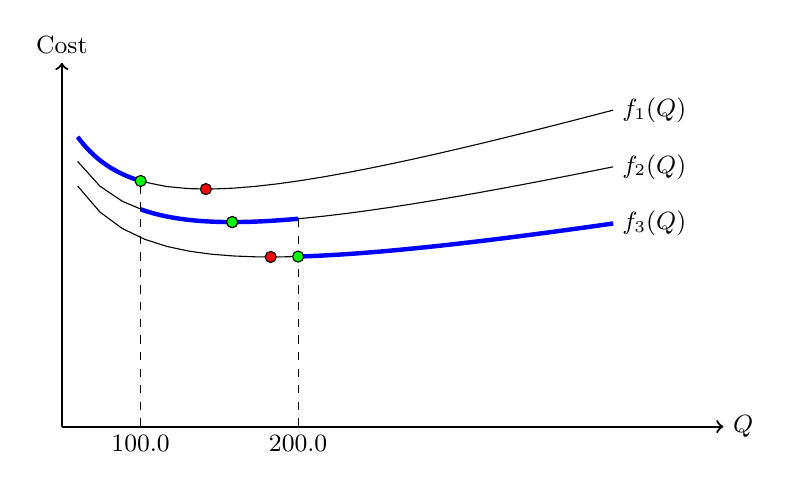
\begin{tikzpicture}[x=0.02cm,y=0.06cm]
\small
\def\c{1} 
\def\K{100} 
\def\h{0.2} 
\def\d{20} 
\def\alpha{0.2}
\def\w{100}
\draw[thick,->] (50,-2) -- (470,-2) node[right] {$Q$};
\draw[thick,->] (50,-2) -- (50,75) node[above] {Cost};
\foreach \n/\c in {1/1.0,2/0.8,3/0.6} {
	\pgfmathsetmacro{\h}{\alpha*\c}	
	\pgfmathsetmacro{\Q}{sqrt(2)*sqrt(\K)*sqrt(\d)/sqrt(\h)}
	\pgfmathsetmacro{\f}{sqrt(2)*sqrt(\K)*sqrt(\d)*sqrt(\h)+\c*\d}	
	\pgfmathsetmacro{\s}{(\n-1)*\w}	
	\pgfmathsetmacro{\e}{\n*\w}

	\draw[domain=60:400] plot (\x,{\d*\K/\x+\c*\d+\h*\x/2}) node[right] {$f_{\n}(Q)$};

	\ifnum\n<3
		\draw[color=blue,ultra thick,domain={max(60,\s}:\e] plot (\x,{\d*\K/\x+\c*\d+\h*\x/2});
		\draw[dashed] (\e,-2) -- (\e,{\d*\K/\e+\c*\d+\h*\e/2});
		\draw (\e,-2) node[below] {$\e$};
	\else
		\draw[color=blue,ultra thick,domain={max(60,\s}:400] plot (\x,{\d*\K/\x+\c*\d+\h*\x/2});
	\fi

	\draw [fill=red] (\Q,\f) circle (2pt);

	\pgfmathparse{int(\Q-\s)}
	\ifnum \pgfmathresult < 0
		\draw [fill=green] (\s,{\d*\K/\s+\c*\d+\h*\s/2}) circle (2pt);
	\fi
	\pgfmathparse{int(\Q-\e)}
	\ifnum \pgfmathresult > 0
		\draw [fill=green] (\e,{\d*\K/\e+\c*\d+\h*\e/2}) circle (2pt);
	\fi
	\pgfmathparse{int((\Q-\e)*(\Q-\s))}
	\ifnum \pgfmathresult < 0
		\draw [fill=green] (\Q,\f) circle (2pt);
	\fi
}
\end{tikzpicture}
\caption{All-unit discounts -- average costs}
\label{fig:avgcost_allunit}
\end{figure}


What we observe here is the following.
\begin{itemize}
\item $f_1(Q)$: This function applies in the $[0,100)$ interval (blue area). It's optimal point is at $141.42$. This point does not fall into function's interval (that's why it is a red dot). Because the function is convex and it's optimal point is to the right of the interval, the minimum point that falls into function's interval is 100 (green dot) which gives a cost of \$50. 
\item $f_2(Q)$: This function applies in the $[100,200)$ interval (blue area). It's optimal point is at $158.11$. This point indeed fall into function's interval (that's why it is a green dot) and it gives a cost of \$41.3. 
\item $f_3(Q)$: This function applies in the $[200,\infty)$ interval (blue area). It's optimal point is at $182.57$. This point does not fall into function's interval (that's why it is a red dot). Because the function is convex and it's optimal point is to the left of the interval, the minimum point that falls into function's interval is 200 (green dot) which gives a cost of \$34. 
\end{itemize}

Based on these observations, we can conclude that the minimum average cost per unit time we can attain is \$34. To achieve that, our order quantity should be 200 units.

Here we followed a simple procedure to find the optimal order quantity. We first devised a cost function for each discount interval. Then, we evaluated the global optimums of these functions and assessed whether those optimal points fall into the associated intervals, and based on that we characterized the best order quantity for each discount interval. Finally, we compared the costs of the optimal points of all functions and found out which one is the best. This procedure can be used to find the optimal order quantity for any problem instance. 

\paragraph{Incremental discounts}

In case of incremental discounts, the procedure we follow is almost the same. But this time we construct the cost function in a different fashion.

First, let us recap the total procurement cost function in case of incremental discounts:
\begin{equation*}
c(Q) = 
\begin{cases}
c_1 Q & \text{if } 0 \leq Q < Q_1 \\
c_1 Q_1 + c_2(Q - Q_1) & \text{if } Q_1 \leq Q < Q_2 \\
\ldots \\
c_1 Q_1 + c_2(Q_2 - Q_1) + \ldots + c_m(Q - Q_{m-1}) & \text{if } Q_{m-1} \leq Q 
\end{cases}
\end{equation*}

Notice that, for each discount interval, only the last term of the expression is dependent on $Q$ and all the rest are just constants. Thus, we can re-write $c(Q)$ in the following form
\begin{equation*}
c(Q) = 
\begin{cases}
\pi_1 + c_1 Q & \text{if } 0 \leq Q < Q_1 \\
\pi_2 + c_2 Q & \text{if } Q_1 \leq Q < Q_2 \\
\ldots \\
\pi_m + c_m Q & \text{if } Q_{m-1} \leq Q 
\end{cases}
\end{equation*}
where $\pi_1=0$ and $\pi_n=\pi_{n-1}+(c_{n-1}-c_n)\,Q_{n-1}$ for all $n>0$.

We also know that we can write the average cost function as 
\begin{align*}
f(Q) = \frac{AD}{Q} + \frac{c(Q)}{Q} D + \frac{\alpha \frac{c(Q)}{Q}Q}{2} = \frac{(A+c(Q))D}{Q} + \frac{\alpha c(Q)}{2} 
\end{align*}
where $\frac{c(Q)}{Q}$ stands for the average procurement cost. 

If we combine the two above, we can write the cost function by conditioning on the order quantity intervals as follows:
\begin{equation*}
f(Q) = 
\begin{cases}
f_1(Q) = \frac{(A+\pi_1)D}{Q} + c_1 D + \frac{\alpha (\pi_1 + c_1 Q)}{2} & \text{if } 0 \leq Q < Q_1 \\
f_2(Q) = \frac{(A+\pi_2)D}{Q} + c_2 D + \frac{\alpha (\pi_2 + c_2 Q)}{2} & \text{if } Q_1 \leq Q < Q_2 \\
\ldots \\
f_m(Q) = \frac{(A+\pi_m)D}{Q} + c_m D + \frac{\alpha (\pi_m + c_m Q)}{2} & \text{if } Q_{m-1} \leq Q 
\end{cases}
\end{equation*}
Here, we have a cost function $f_n(Q) = \frac{(A+\pi_n)D}{Q} + c_n D + \frac{\alpha (\pi_n + c_n Q)}{2}$ for each interval $n$ which only applies if the order quantity $Q$ is in $[Q_{n-1},Q_n)$. This function has the same mathematical properties with the original EOQ formula. There are yet two differences: first we have an $A+\pi_n$ term rather than $A$ and second we have a new constant term $\frac{\alpha \pi_n}{2}$. Therefore, we know that $f_n(Q)$ is minimized at $Q^*_n=\sqrt{\frac{2(A+\pi_n)D}{\alpha c_n}}$ and its minimum value is $f_n(Q^*_n)=\sqrt{2(A+\pi_n)D\alpha c_n}+c_n D+\frac{\alpha \pi_n}{2}$.

Let us illustrate this by once again considering the example from the previous exercise where $c_1=1.0$, $c_2=0.8$, $c_3=0.6$, $Q_1=100$, and $Q_2=200$. We further let $A=100$, $D=20$, and $\alpha=0.2$. 

First, we compute $\pi_1=0$, $\pi_2=20$, and $\pi_3=60$. Then we have
\begin{equation*}
f(Q) = 
\begin{cases}
f_1(Q) = \frac{2000}{Q} + 20 + 0.10 Q & \text{if } 0 \leq Q < Q_1 \\
f_2(Q) = \frac{2400}{Q} + 18 + 0.08 Q & \text{if } Q_1 \leq Q < Q_2 \\
f_3(Q) = \frac{3200}{Q} + 18 + 0.06 Q & \text{if } Q_{2} \leq Q 
\end{cases}
\end{equation*}
and we also know $Q^*_1\approx 141.42$, $Q^*_2\approx 173.21$, and $Q^*_3\approx 230.94$. 

In Figure~\ref{fig:avgcost_incremental} we draw all these functions.

\begin{figure}[htbp]
\centering
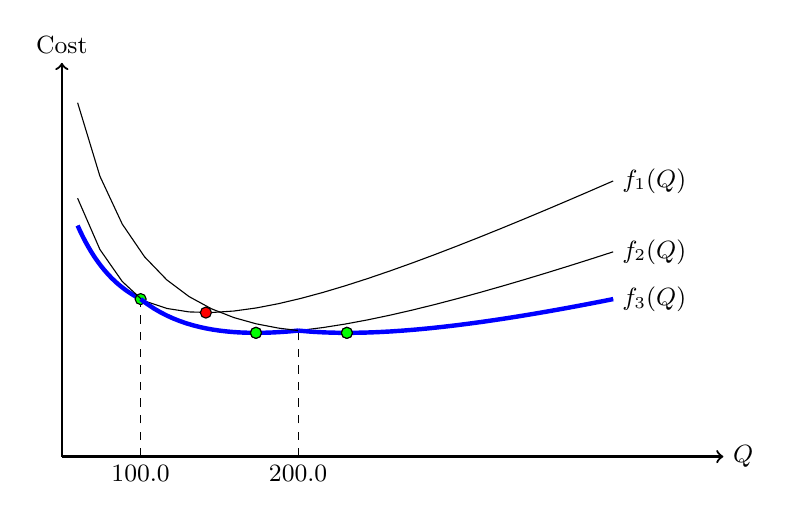
\begin{tikzpicture}[x=0.02cm,y=0.10cm]
\small
\def\c{1} 
\def\K{100} 
\def\h{0.2} 
\def\d{20} 
\def\alpha{0.2}
\def\w{100}
\draw[thick,->] (50,30) -- (470,30) node[right] {$Q$};
\draw[thick,->] (50,30) -- (50,80) node[above] {Cost};
\foreach \n/\a/\b/\c in {1/2000/20/0.1,2/2400/18/0.08,3/3200/18/0.06} {
	\pgfmathsetmacro{\Q}{sqrt(\a)/sqrt(\c)}	
	\pgfmathsetmacro{\f}{\a/\Q+\b+\c*\Q}	
	\pgfmathsetmacro{\s}{(\n-1)*\w}	
	\pgfmathsetmacro{\e}{\n*\w}

	\draw[domain=60:400] plot (\x,{\a/\x+\b+\c*\x}) node[right] {$f_{\n}(Q)$};

	\ifnum\n<3
		\draw[color=blue,ultra thick,domain={max(60,\s}:\e] plot (\x,{\a/\x+\b+\c*\x});
		\draw[dashed] (\e,30) -- (\e,{\a/\e+\b+\c*\e});
		\draw (\e,30) node[below] {$\e$};
	\else
		\draw[color=blue,ultra thick,domain={max(60,\s}:400] plot (\x,{\a/\x+\b+\c*\x});
	\fi

	\draw [fill=red] (\Q,\f) circle (2pt);

	\pgfmathparse{int(\Q-\s)}
	\ifnum \pgfmathresult < 0
		\draw [fill=green] (\s,{\a/\s+\b+\c*\s}) circle (2pt);
	\fi
	\pgfmathparse{int(\Q-\e)}
	\ifnum \pgfmathresult > 0
		\draw [fill=green] (\e,{\a/\e+\b+\c*\e}) circle (2pt);
	\fi
	\pgfmathparse{int((\Q-\e)*(\Q-\s))}
	\ifnum \pgfmathresult < 0
		\draw [fill=green] (\Q,\f) circle (2pt);
	\fi
}
\end{tikzpicture}
\caption{Incremental discounts -- average costs}
\label{fig:avgcost_incremental}
\end{figure}


What we observe here is the following.
\begin{itemize}
\item $f_1(Q)$: This function applies in the $[0,100)$ interval (blue area). It's optimal point is at $141.42$. This point does not fall into function's interval (that's why it is a red dot). Because the function is convex and it's optimal point is to the right of the interval, the minimum point that falls into function's interval is 100 (green dot) which gives a cost of \$50. 
\item $f_2(Q)$: This function applies in the $[100,200)$ interval (blue area). It's optimal point is at $173.21$. This point indeed fall into function's interval (that's why it is a green dot) and it gives a cost of \$45.7. 
\item $f_3(Q)$: This function applies in the $[200,\infty)$ interval (blue area). It's optimal point is at $230.94$. This point indeed fall into function's interval (that's why it is a green dot) and it gives a cost of \$45.7.  
\end{itemize}

Based on these observations, we can conclude that the minimum average cost per unit time we can attain is \$45.7. To achieve that, our order quantity should either be 173.21 units or 230.94 units.
\end{solution}

\begin{question}
We have thus far only considered environments where inventories are replenished from an external source. Does the EOQ model apply to production environments?
\end{question}

\begin{solution}
It does. This version of the EOQ is often referred to as the EPQ (Economic Production Quantity) model. The difference between EOQ and EPQ models lies in how they treat replenishments:
\begin{enumerate}
\item The EOQ model assumes that the order arrive all at once.
\item The EPQ model assumes that once production is switched on items are produced on a continuous basis with a fixed rate.
\end{enumerate}
\end{solution}

\begin{question}
Explain the inventory policy behind the EPQ model. What are its parameters? How does it work?
\end{question}

\begin{solution}
The policy works as follows. We switch on production when the inventory level hits zero. Then we produce $Q$ units and then we switch off. The policy thus have a single parameter $Q$, i.e. production quantity in one replenishment cycle. 
\end{solution}

\begin{question}
Illustrate how the inventory behaves over time for the EPQ model. Then write down the cost function and characterize the optimal policy parameters.
\end{question}

\begin{solution}

See Figure~\ref{fig:EPQ}.

\begin{figure}[htbp]
\centering
\small
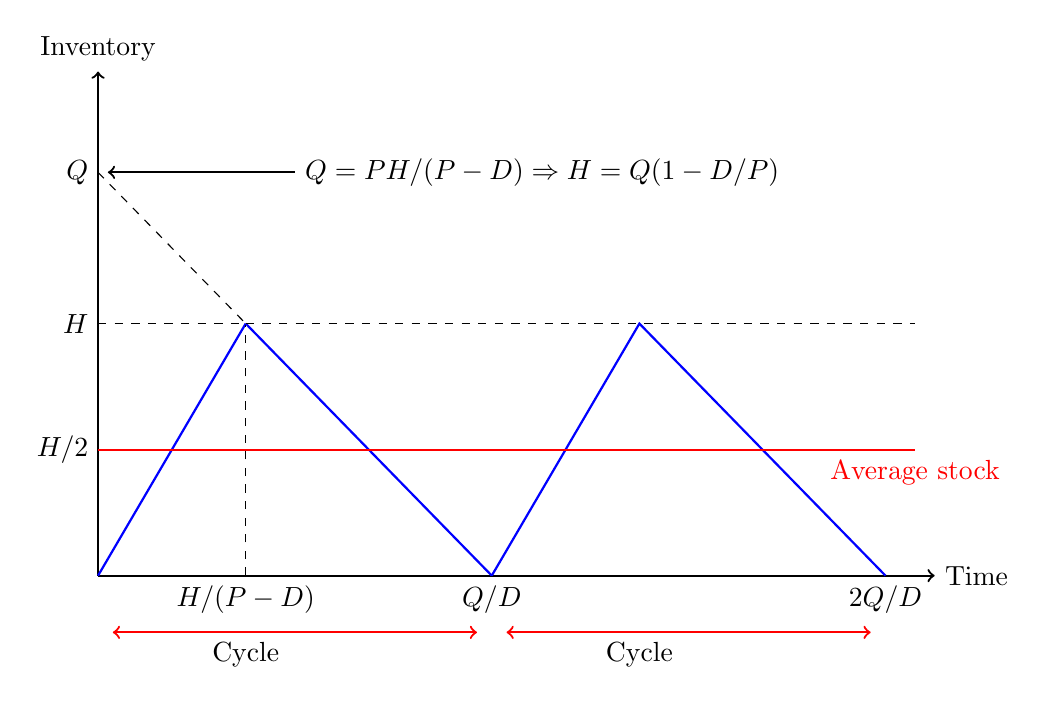
\begin{tikzpicture}[x=1.25cm,y=0.016cm]
\draw[thick,->] (0,0) -- (8.5,0) node[right] {Time};
\draw[thick,->] (0,0) -- (0,400) node[above] {Inventory};
\draw[] (0,200) node[left] {$H$};
\draw[dashed] (0,200) -- (1.5,200);
\draw[color=blue,thick] (0,0) -- (1.5,200);
\draw[] (1.5,0) node[below] {$H / (P-D)$};
\draw[dashed] (1.5,0) -- (1.5,200);
\draw[color=blue,thick] (1.5,200) -- (4,0);
\draw[dashed] (0,4*200/2.5) -- (1.5,200);
\draw[] (0,4*200/2.5) node[left] {$Q$};
\draw[] (4,0) node[below] {$Q / D$};
\draw[thick,<-] (0.1,4*200/2.5) -- (2,4*200/2.5) node[right] {$Q = PH / (P - D) \Rightarrow  H = Q(1 - D / P)$};
\draw[dashed] (1.5,200) -- (8.3,200);
\draw[color=blue,thick] (4,0) -- (4+1.5,200) -- (8,0);
\draw[] (8,0) node[below] {$2Q / D$};
\draw[] (0,100) node[left] {$H / 2$};
\draw[color=red,thick] (0,100) -- (8.3,100) node[below] {Average stock};
\foreach \y in {0,...,1}{
	\draw[color=red,thick,<->] (4*\y+0.15,-45) -- (4*\y+4-0.15,-45);
	\draw[] (4*\y+1.5,-45) node[below] {Cycle};}
\end{tikzpicture}
\caption{EPQ model}
\label{fig:EPQ}
\end{figure}


It is important to observe that the inventory behaves differently when production is on and off. If production is on, then the inventory increases with the rate $P-D$. Here $P$ stands for the production rate i.e. number of items produced in unit time. Note that $P$ is supposed to be larger than $D$, as it would otherwise be impossible to cover the demand. If production is off, the inventory process is the same with the classical model where it decreases with rate $D$. The production quantity in one cycle is $Q$. At the beginning of each cycle, production is switched on and it is switched off once $Q$ items have been produced. Because the inventories increase with rate $P-D$ during that time, we end up with $H=Q(1-\frac{D}{P})$ units once the machine has been turned off. Then production remains off until the inventory level drops down to zero, and then another cycle starts.

The total cost for one cycle is the sum of ordering cost, procurement cost, and inventory (holding) cost. The fixed setup cost (rather than fixed ordering) is $A$ per cycle as we switch on the machine only once in each cycle. The production cost (rather than procurement) equals the unit production cost times the order quantity $cQ$, i.e. we produce just enough to satisfy all the demand in each cycle. The inventory cost per cycle is the total area of the triangle times $h$, i.e. 
\begin{equation*}
h~\frac{\text{height}\cdot\text{base}}{2} = h~\frac{H \cdot Q/D }{2} = \left(1-\frac{D}{P}\right) \frac{h Q^2}{2D}.
\end{equation*}

Thus, the total cycle cost is $A+cQ+\frac{(1-\frac{D}{P}) h Q^2}{2D}$. The average cost per unit time is this total cost divided by the duration of one cycle, which is $\frac{Q}{D}$. Therefore, the average cost is
\begin{equation*}
A \frac{D}{Q}+cQ \frac{D}{Q} + \left(1-\frac{D}{P}\right) \frac{h Q^2}{2D} \frac{D}{Q} = \frac{AD}{Q}+cD+\left(1-\frac{D}{P}\right)\frac{hQ}{2}
\end{equation*}

This expression gives us the average cost as a function of the order quantity:
\begin{equation*}
f(Q) = \frac{AD}{Q}+cD+\left(1-\frac{D}{P}\right)\frac{hQ}{2}.
\end{equation*}

It is easy to observe at this point that we can derive the average cost function of the EPQ model simply by revising the holding cost $h$ of the EOQ model as $h'=h \left(1-\frac{D}{P}\right)$. All relevant results, such as expressions of the optimal order quantity and cost then immediately follows. For instance, the optimal production quantity $Q^*=\sqrt{\frac{2AD}{h'}}$ and optimal average cost per unit time $f(Q^*)=\sqrt{2ADh'}+cD$. The intuition behind is as follows. Let us assume that we are using the same $Q$ for the EOQ and EPQ models. Then the average stock level and thus the holding costs of the EPQ model will be $1-\frac{D}{P}$ times the average stock level of the EOQ model, and all other costs will be the same.  
\end{solution}

\begin{question}
For which parameter settings the optimal policies EOQ and EPQ models have a similar structure? 
\end{question}

\begin{solution}
Recall that the main difference between EOQ and EPQ models is that EOQ assumes the order arrive all at once and EPQ assumes items are produced with a fixed rate. Let us consider the EPQ model and assume that the production rate is extremely high. Then production becomes almost instantaneous. This setting should yield the same results with the EOQ model.

This is obvious if we look at the average cost function $f(Q) = \frac{AD}{Q}+cD+\frac{h'Q}{2}$ where $h'=h\left(1-\frac{D}{P}\right)$. If $P$ is very large, then 
$\left(1-\frac{D}{P}\right)$ approaches 1. Then $h'\approx h$ and we have the same cost function. For moderate values of $P$ the expression $\left(1-\frac{D}{P}\right)$ will be in between 0 and 1. Then $h'<h$ and it implies that the EPQ function is lower than the EOQ function.
\end{solution}

\begin{question}
How does the production rate affect the optimal production quantity and the average cost per unit time?
\end{question}

\begin{solution}
Let us consider the optimal production quantity $Q^*=\sqrt{\frac{2AD}{h'}}$ and corresponding optimal average cost per unit time $f(Q^*)=\sqrt{2ADh'}+cD$ where $h'=h\left(1-\frac{D}{P}\right)$. It is clear that the smaller the $P$ the smaller the adapted holding cost $h$. Then it is easy to see that a higher production rate leads to a smaller $Q^*$ and a higher $f(Q^*)$. 

We know that the production rate should be larger than the demand rate to be able to cover demand over time. Thus, the lowest feasible production rate is the demand rate itself. In this case we have $P=D$ and therefore $h'=h\left(1-\frac{D}{D}\right)=0$. The mathematics of this particular case is ill-defined to the division by 0. Nevertheless, it is easy to see what is going on. Because the production rate equals the demand rate; we simply have is no inventory! We switch on the machine and leave it switched on all the time. Thus we have neither fixed setup cost nor holding cost. All we need to pay is the production cost which is $cD$ per unit time.
\end{solution}

\begin{question}
It appears that having a slower production rate is favorable. How does this makes sense?
\end{question}
\begin{solution}
The issue is with the trade-off between setup and holding costs. If the machine is fast, then once you switch on you quickly build up inventories at a high speed. To avoid excessive inventories you switch off. But then you pay the setup cost more frequently. 
\end{solution}


\subsection{ELS and Extensions}

The EOQ model has rather strict assumptions on the demand. Probably one of the most restrictive ones among those is demand being stationary, or in other words time-invariant.

The most well-known deterministic inventory model with time-varying demands is the ELS (Economic Lot Sizing) model. In the following exercises we first go through the standard ELS model and then we modify its assumptions to investigate how the environment affects this inventory model. 

\begin{question}
We know that often in real-life the demand change over time. How can we capture that in inventory management.
\end{question}

\begin{solution}
We need to use an approach to explain how demand evolve over time. For instance, let $D(t)$ be the demand at time $t$ and assume that the process starts with no demand, i.e. $D(0)=0$, and then it increases over time with some rate $a$ per unit time. Then we can write $D(t)=at$. However, this way of modeling demand is not very handy with respect to inventory management as the mathematics to compute costs would involve nasty integrals. 

A practical alternative is to approach time in a discrete fashion, i.e. to count time as a discrete entity such as days, weeks, or months. This allows us to express the demand in period $n$ as a scalar such as $D_n$. Because time is now discrete, the way that the costs are accounted for should be different. The conventional approach is to do the cost accounting at the end of the periods. Here, the sequence of events in a period are as follows: (1) we observe the inventory level from the previous period, (2) we make a replenishment decision and (if applicable) pay the fixed ordering and procurement costs, (3) if an order is placed then it is received (assuming no lead time -- otherwise we receive the order from $L$ period before), (4) demand is realized, and (5) inventory costs are charged for the inventories at the end of the period. Observe that this is different than the continuous-time cost accounting. In discrete time cost accounting, in each period holding costs are charged only once. In continuous time cost accounting, holding cost are charged at all times. Long story short, we do not have the triangles any more! We rather have a bar for each period! 
\end{solution}

\begin{question}
How time-varying demands effect the replenishment policy?
\end{question}

\begin{solution}
It is simple. If demands are time-varying the replenishment quantities should also be time-varying. That is, the order quantity in different periods should also be different. 
\end{solution}

\begin{question}
How can we devise an inventory model if time is modeled as discrete periods and demands are known for each time periods?
\end{question}

\begin{solution}
To begin with, we assume that stock-outs are not permitted and total costs are comprised of fixed replenishment costs procurement costs, and holding costs. We will devise a model to compute the total cost over a finite planning horizon.

We begin with inventory dynamics. Let $Q_n$ be the order quantity in period $n$ and $I_n$ be the inventory level at the end of period $n$. Then we immediately have $I_n=I_{n-1}+Q_n-D_n$. Here, if $Q_n=0$ then we do not place an order. In this case, we only have the holding cost in period $n$. This can be written as $h\cdot I_n$. Note that the unit holding cost $h$ should be scaled for the time period. That is, if we count time in days, then $h$ should be the unit holding cost per day. If $Q_n>0$ then we place an order. In this case, we have fixed ordering and procurement costs as well as the holding cost in period $n$. This can be written as $A+c\cdot Q_n+h\cdot I_n$.

Now let us assume that there are $T$ periods in the planning horizon. If ordering quantities are $Q_1,Q_2,\ldots,Q_T$, then we can construct an expression for the total cost over the planning horizon as follows:
\begin{align*}
\sum_{n=1}^T A \1{Q_n} + c Q_n + hI_n
\end{align*}
\end{solution}

\begin{question}
How can we implement the DLS model? Illustrate through an example where $A=54$ and $h=0.4$, with demands $\{10,62,12,130,154,129,88,52,124,160,238,41\}$ over a 12-period planning horizon, and assume that we place an order of size 300 every three periods. 
\end{question}

\begin{solution}
This model can easily be implemented in a spreadsheet. The inventories and costs associated with each period are provided in Figure~\ref{fig:3300}. The total cost of this replenishment policy is \$2412.8.

\begin{figure}[htbp]
\begin{subfigure}[b]{0.5\textwidth}
  \centering
    \begin{tabular}{rrrrr}
    \toprule
          & $D$ & $Q$ & $I$ & Cost \\
	\midrule
    1     & 10    & 300   & 290   & 470 \\
    2     & 62    &       & 228   & 91.2 \\
    3     & 12    &       & 216   & 86.4 \\
    4     & 130   & 300   & 386   & 508.4 \\
    5     & 154   &       & 232   & 92.8 \\
    6     & 129   &       & 103   & 41.2 \\
    7     & 88    & 300   & 315   & 480 \\
    8     & 52    &       & 263   & 105.2 \\
    9     & 124   &       & 139   & 55.6 \\
    10    & 160   & 300   & 279   & 465.6 \\
    11    & 238   &       & 41    & 16.4 \\
    12    & 41    &       & 0     & 0 \\
    \bottomrule
    \end{tabular}%
\caption{Order 300 unit every three periods}
\label{fig:3300}
\end{subfigure}
~
\begin{subfigure}[b]{0.5\textwidth}
  \centering
    \begin{tabular}{rrrrr}
    \toprule
          & $D$ & $Q$ & $I$ & Cost \\
	\midrule
    1     & 10    & 84    & 74    & 167.6 \\
    2     & 62    &       & 12    & 4.8 \\
    3     & 12    &       & 0     & 0 \\
    4     & 130   & 413   & 283   & 580.2 \\
    5     & 154   &       & 129   & 51.6 \\
    6     & 129   &       & 0     & 0 \\
    7     & 88    & 264   & 176   & 388.4 \\
    8     & 52    &       & 124   & 49.6 \\
    9     & 124   &       & 0     & 0 \\
    10    & 160   & 439   & 279   & 604.6 \\
    11    & 238   &       & 41    & 16.4 \\
    12    & 41    &       & 0     & 0 \\
    \bottomrule
    \end{tabular}%
\caption{Order for the cycle every three periods}
\label{fig:3just}
\end{subfigure}
\caption{Ad-hoc solutions to the ELS model}
\end{figure}
\end{solution}


\begin{question}
It appears from the resulting cost figures that it may not be the best option to to have inventories right before placing an order. Is it always the case? 
\end{question}

\begin{solution}
Yes. There is no incentive in the DLS model to carry inventories from one replenishment cycle to the next. This is often referred to as the 'zero-inventory' property. Let us revise our order quantities in the previous example to account for this property. That is, we still order every three periods, but this time the order we place will be exactly sufficient to cover demands in the next three periods. The inventories and costs associated with each period are provided in Figure~\ref{fig:3just}. Notice that the inventory level drops down to zero in every three periods. The total cost of this replenishment policy is \$1863.2. This is much better than the previous example.
\end{solution}

\begin{question}
How do we find the best order quantities in the DLS model?
\end{question}

\begin{solution}
There are many procedures for this purpose. One efficient procedure is the Wagner-Whitin algorithm. This algorithm explained in detail in FP Section 2.3.3. We do not go over that here.

Another approach is to model and solve the problem as a MIP (Mixed Integer Program). Then we can easily solve it using a spreadsheet application rather than coding an algorithm. The MIP model of the DLS can be written as follows:
\begin{align*}
\min\quad 
	& \sum_{n=1}^T \left\{Ay_n + hI_n\right\} \\
\sto\quad
	& I_n = I_{n-1} + Q_n - d_n \quad n\in 1,\ldots,T \\
	& Q_n \leq M y_n \quad n\in 1,\ldots,T \\
	& I_0 = 0 \\
	& y_n \in \{0,1\}, Q_n, I_n \in \mathbb{R}_+ \quad n\in 1,\ldots,T
\end{align*}
Here, we have three sets of decision variables; $y_n$ is a binary (zero-one) variable that indicates whether an order is placed in period $n$, and $Q_n$ and $I_n$ are continuous and non-negative variables that stand for the order quantity and inventory level in period $n$. The objective function sums total costs over the planning horizon. The costs are comprised of the fixed ordering cost $Ay_n$ (if $y_n=0$ there is no ordering cost, otherwise it is $A$) and holding costs $hI_n$. The first constraint specifies inventory conservation over periods. The second constraint makes sure that $Q_n$ can only be non-zero if $y_n=1$. Here, $M$ is a sufficiently large constant (say total demand over the planning horizon). It constitutes an upper bound on the order quantity. The constraint simply states that if $y_n=0$ then $Q_n=0$ as well. The third constraint specifies the inventory level at the beginning of the planning horizon. Here it is assumed to be zero, but it can be replaced with any other inventory level. The fourth constraint specifies the domains of decision variables.

It is important to note that the cost parameters such as fixed ordering cost $A$, procurement cost $c$, and holding cost $h$ can also be time-varying, i.e. $A_n,c_n.h_n$. These can easily be embedded into the model above.

The MIP model can be easily implemented in a spreadsheet. If we use this model for the running example, we obtain the inventories and costs provided in Figure~\ref{fig:LS_opt}. The total cost of this replenishment policy is \$1701.2. This is the minimum cost that can possibly be attained for this example.

\begin{figure}[htbp]
\begin{subfigure}[b]{0.5\textwidth}
  \centering
    \begin{tabular}{rrrrr}
    \toprule
          & $D$ & $Q$ & $I$ & Cost \\
	\midrule
    1     & 10    & 84    & 74    & 167.6 \\
    2     & 62    & 0     & 12    & 4.8 \\
    3     & 12    & 0     & 0     & 0 \\
    4     & 130   & 130   & 0     & 184 \\
    5     & 154   & 283   & 129   & 388.6 \\
    6     & 129   & 0     & 0     & 0 \\
    7     & 88    & 140   & 52    & 214.8 \\
    8     & 52    & 0     & 0     & 0 \\
    9     & 124   & 124   & 0     & 178 \\
    10    & 160   & 160   & 0     & 214.0 \\
    11    & 238   & 279   & 41    & 349.4 \\
    12    & 41    & 0     & 0     & 0 \\
    \bottomrule
    \end{tabular}%
\caption{Optimal solution}
\label{fig:LS_opt}
\end{subfigure}
~
\begin{subfigure}[b]{0.5\textwidth}
  \centering
    \begin{tabular}{rrrrr}
    \toprule
          & $D$ & $Q$ & $I$ & Cost \\
	\midrule
    1     & 10    & 10    & 0     & 64 \\
    2     & 62    & 74    & 12    & 132.8 \\
    3     & 12    &       & 0     & 0 \\
    4     & 130   & 130   & 0     & 184 \\
    5     & 154   & 423   & 269   & 584.6 \\
    6     & 129   &       & 140   & 56 \\
    7     & 88    &       & 52    & 20.8 \\
    8     & 52    &       & 0     & 0 \\
    9     & 124   & 124   & 0     & 178 \\
    10    & 160   & 160   & 0     & 214 \\
    11    & 238   & 279   & 41    & 349.4 \\
    12    & 41    &       & 0     & 0 \\
    \bottomrule
    \end{tabular}%
\caption{Silver-Meal solution}
\label{fig:LS_SM}
\end{subfigure}
\caption{Optimal and Wagner-Whitin solutions to the ELS model}
\end{figure}
\end{solution}


\begin{question}
The spreadsheet application has taken quite a bit of time to solve this model. Is there a simple way to obtain a high quality solution for the DLS?
\end{question}

\begin{solution}
There are many different MIP formulations in the literature designed to solve the DLS model. Some of them are much more efficient than the one we presented here, yet they are still easy to implement. But we leave that to you as it is not the place to delve into the details of more efficient MIP models.

There are also good heuristic approaches. One that definitely needs mentioning is the Silver-Meal heuristic. This is a myopic heuristic in the sense that it requires only a few periods of demand information to make a replenishment decision in the actual period. It is based on the idea of finding replenishment cycles with the least cost per period. 

Let $f(n,a)$ be the average cost per period over periods $\{n,n+1,\ldots,n+a\}$ if an order is placed in period $n$ to cover the demand in these periods, i.e. next replenishment will take place in period $n+a+1$. This can be computed as
\begin{align*}
f(n,a) 
& = \frac{A + (c+0\cdot h) \cdot D_{n} + (c+1\cdot h)\cdot D_{n+1} + (c+2\cdot h)\cdot D_{n+2} + \ldots + (c+a\cdot h)\cdot D_{n+a}}{a+1} \\
& = \frac{A + \sum_{k=0}^a \left((c+k\cdot h)\cdot D_{n+k}\right)}{a+1}.
\end{align*}

In a nutshell the algorithm works as follows. If we are given an arbitrary period $n$, we sequentially compute $f(n,0),f(n.1),\ldots$ as long as the newly computed value is smaller than the previous one. If not, we stop. Let $a$ be the where we stop. Then we conclude that the next cycle starts at period $n+a+1$. The algorithm is implemented starting from period 1 and in each step we find the next replenishment period until we reach the end of the planning horizon.

If we use the Silver-Meal heuristic for the running example, we obtain the inventories and costs provided in Figure~\ref{fig:LS_SM}. The total cost of this replenishment policy is \$1783.6. This is very close to the minimum cost solution obtained by MIP. \textit{\textbf{Note:} This solution does not exactly match with the one we saw in the lecture. Do you have an idea why?}
 
\end{solution}

\begin{question}
How can we account for capacity limitations in the ELS model? Let's say there is a limit on the amount that we can order each month.
\end{question}

\begin{solution}
This is a non-trivial extension in general. For instance, Wagner-Whitin algorithm and Silver-Meal heuristic cannot account for this case. There are other algorithms but again this is not the place. Having said that it is very easy to adapt the MIP model to account for capacity limitations. Let us assume the upper bound on the order quantity is $C$ in each period. We only need to re-write the the second constraint so that $Q_n$ does not exceed $C$ even when $y_n=1$. This can be done by replacing $M$ with $C$ as 
\begin{align*}
	& Q_n \leq C y_n \quad n\in 1,\ldots,T.
\end{align*}
\end{solution}

\begin{question}
Is it also possible to have more sophisticated capacity constraints. For instance, what if we can order at most $C$ units in three consecutive periods?
\end{question}

\begin{solution}
We can add the following constraint in the MIP model:
\begin{align*}
	& Q_n + Q_{n+1} + Q_{n+2} \leq C \quad n\in 1,\ldots,T-2.
\end{align*}
\end{solution}

\begin{question}
Let us consider a case where we pay the fixed ordering cost for the container in which supplies are brought from overseas. Here, fixed ordering cost can be shared among a number of products. Thus. if we are planning to place an order anyway we might want to add many different types of products into the order. The ELS models we have seen thus far only consider single-item inventory control problems. How can we extend the ELS model to account for multi-item systems such as the one described here? 
\end{question}

\begin{solution}
In principle, multi-item systems with shared fixed costs are challenging. They are often referred to as 'joint replenishment' problems. We can account for such a problem by means of MIP; by extending the single-item model to multi-items. This can be done as follows:
\begin{align*}
\min\quad 
	& \sum_{n=1}^T \left\{A y_n + \sum_{k=1}^K h I_{kn}\right\} \\
\sto\quad
	& I_{kn} = I_{kn-1} + Q_{kn} - d_{kn} \quad k\in 1,\ldots,K; n\in 1,\ldots,T \\
	& \sum_{k=1}^K Q_{kn} \leq C y_n \quad n\in 1,\ldots,T \\
	& I_{k0} = 0 \quad k\in 1,\ldots,K \\
	& y_n \in \{0,1\}, Q_{kn}, I_{kn} \in \mathbb{R}_+ \quad k\in 1,\ldots,K; n\in 1,\ldots,T
\end{align*}

Nevertheless, solving such a model is computationally much more expensive as compared to it's single-item counterpart.

 
\end{solution}

%
%%
%%
%%
%%\begin{question}
%%EOQ with joint ordering
%%  \begin{solution}
%%    TBD
%%  \end{solution}
%%\end{question}
%%
%%\begin{question}
%%  Consider the setting of the EOQ model but now with batchsize
%%  constraints, that is, the order quantity is in multiples of some number $q$, say. Can you make a formula for the cost, and find the minimum?
%%  \begin{solution}
%%This is, in fact, really easy. Suppose we order $n$ times the minimal order quantity $q$. Then, for a yearly demand $D$, ordering cost $A$, and inventory cost $h$, we pay per year
%%\begin{equation*}
%%  A \frac{D}{nq} + h\frac{nq}2 = A\frac{D/q}n + hq\frac{n}2.
%%\end{equation*}
%%But this is precisely the normal EOQ model with demand $D'=D/q$ and inventory cost $h'=hq$. Thus, the optimal number of batches to order is:
%%\begin{equation*}
%%  n^2 = \frac{2D'A}{h'} = \frac{2AD/q}{hq} = \frac{2AD}{hq^2}.
%%\end{equation*}
%%Hence, the optimal $n$ expressed in the EOQ quantity $Q^*$ is 
%%\begin{equation*}
%%  n = \sqrt{\frac{2AD}{h}}\frac1q=\frac{Q^*}q.
%%\end{equation*}
%%  \end{solution}
%%\end{question}
%%
%%
%%\begin{question}
%%EOQ with yield loss
%%  \begin{solution}
%%    TBD
%%  \end{solution}
%%\end{question}
%%
%%\begin{question}
%%EOQ with lower salvage value
%%  \begin{solution}
%%    TBD
%%  \end{solution}
%%\end{question}
%%
%%
%%\begin{question}
%%EOQ with constraints on cycle length
%%
%%EOQ under periodic review rather than continuous review.
%%
%%Constraints on when to order, order moment.
%%
%%  \begin{solution}
%%    TBD
%%  \end{solution}
%%\end{question}
%%
%%
%%\begin{question}
%%  EOQ with positive replenishment lead time and variance in the lead
%%  time.
%%
%%  \begin{solution}
%%    TBD
%%
%%Suddenly we have to deal with safety stock!
%%  \end{solution}
%%\end{question}
%%
%%\begin{question}
%%  Suppose that the delivery rate of the items we order is not
%%  `infinite', as it is in the EOQ setting (recall, in the EOQ we
%%  assume instantaneous deliveries). If we have a machine that
%%  replenishes the FGI we have to take into account the production
%%  rate, $r$ say. If it costs $K$ to switch on the machine, when do you switch the machine on or off?
%%  \begin{solution}
%%    An easy policy is to switch the machine on when the FGI level hits
%%    some level $Q$, and switch it off when the level is $0$. Of course
%%    we need to assume that $D<r$, i.e., the production rate is larger
%%    than the demand rate $D$. 
%%
%%    To find an expression to cover this situation we can reason like
%%    this.  When the machine is on, inventory increases at rate
%%    $r-D$. If we keep it on for $T$ time units, then the inventory
%%    level is $T(r-D)$ when we switch off. The time until the inventory
%%    hits 0 is then $T(r-D)/D$, since we start with an inventory level
%%    $T(r-D)$ after switching off and the demand rate is $D$. Thus, the total cycle length is
%%    \begin{equation*}
%%      T + \frac{T(r-D)}D = T + T(\frac{r}D-1) = T + T\frac r D - T = T\frac r D.
%%    \end{equation*}
%%
%%    What is, in the EOQ, the average inventory cost? It is half the
%%    maximal height times $h$, i.e., $hQ/2$. In our present case, the
%%    maximal height is $T(r-D)$. Thus the average inventory cost must
%%    be  $hT(r-D)/2$. 
%%
%%    The ordering cost in the EOQ is $A$ times the order frequency, i.e., $A D/Q$. Here the time between two `order' moments (switching moments) is $Tr/D$. Hence, the frequency is $D/rT$ and the average switching cost is $K D/rT$. 
%%
%%All in all we get for the average cost
%%\begin{equation*}
%%  \frac{h(r-D)}2 T + \frac{K}r \frac DT.
%%\end{equation*}
%%This is similar to the EOQ model with $h'=h(r-D)$ and $A=K/r$. But then the optimal $T$ must be given by
%%\begin{equation*}
%%  T = \sqrt{\frac{2AD}{h'}} = \sqrt{\frac{2DK/r}{h(r-D)}}=\sqrt{\frac{2DK}{hr(r-D)}}.
%%\end{equation*}
%%  \end{solution}
%%\end{question}
%%
%%
%%\begin{question}
%%EOQ with variable demand.
%%  \begin{solution}
%%    TBD
%%  \end{solution}
%%\end{question}
%%
%%\begin{question}
%%Wagner Whitin
%%  \begin{solution}
%%    TBD
%%  \end{solution}
%%\end{question}
%%
%%\begin{question}
%%Silver meal
%%  \begin{solution}
%%    TBD
%%  \end{solution}
%%\end{question}
%%
%%\begin{question}
%%Where to put the I/O interface? For what product/item?
%%  \begin{solution}
%%    TBD
%%  \end{solution}
%%\end{question}
%%
%%\begin{question}
%%  What is the difference between continuous and period review? Why/when to prefer one over the other?
%%  \begin{solution}
%%    TBD
%%  \end{solution}
%%\end{question}
%%
%%\begin{question}
%%  What is the difference between fixed order and order-up-to policies?
%%  Why/when to prefer one over the other?
%%  \begin{solution}
%%    TBD
%%
%%Order quantities
%%
%%  \end{solution}
%%\end{question}
%%
%%\begin{question}
%%  What  different type of service level can you define?
%%  Why/when to prefer one over the other?
%%  \begin{solution}
%%    TBD
%%
%%e.g. cycle service level.
%%  \end{solution}
%%\end{question}
%%
%%\begin{question}
%%  Why to use safefy stock? What is it? 
%%  \begin{solution}
%%    TBD
%%  \end{solution}
%%\end{question}
%%
%%\begin{question}
%%  Are lead times typically (approximately) constant ore variable?
%%  \begin{solution}
%%    TBD
%%  \end{solution}
%%\end{question}
%%
%%
%%
%%\subsection{Strategic impact of short leadtimes/small inventories,
%%  what if lead time is a control?}
%%
%%You run a pharmaceutical company. The medicines you sell need to be
%%packaged. The price quotation of the company that prints the packages
%%depends on the order size $Q$.
%%  \begin{itemize}
%%  \item If $Q$ covers 2 weeks of demand: price per unit is 1.15 Euro
%%  \item If $Q$ covers 1 month of demand: price per unit is 1. Euro
%%  \item If $Q$ covers 2 months of demand: price per unit is 0.95 Euro
%%  \item If $Q$ covers 3 months of demand: price per unit is 0.9 Euro
%%  \item If $Q$ covers 6 months of demand: price per unit is 0.85 Euro
%%  \end{itemize}
%%The problem is to determine how much to order.
%%
%%\begin{question}
%%  \begin{itemize}
%%  \item Include your own storage cost, i.e., packages need to be
%%    stored as your raw materials inventory.  Suppose the
%%    inventory cost is $20\%$ per unit per year. Can we now compute the
%%    inventory cost?  Assume that $D = 12000$ units per year.
%%  \item Include transportation cost.  Assume that $A = 50$ Euro.
%%  \end{itemize}
%%\end{question}
%%
%%\begin{question}
%%Every so often government regulations change. As a result, the entire
%%stock becomes obsolete. What now?
%%\begin{solution}
%%  \begin{itemize}
%%  \item Use data to make assumptions on the probability that the
%%    remaining stock will be affected by a regulation change.
%%  \item Assume that a regulation change occurs, on average, every
%%    month, and time to implement the change is one month.
%%  \item If  $Q$ is 2 weeks of demand, then?  there is no problem
%%  \item If $Q$ is 3 months of demand, then? 
%%  \end{itemize}
%%Challenge: Can you compute the optimal order quantity in this situation? 
%%
%%%   \begin{lstlisting}%{python}
%%% A = 50.
%%% D = 12000
%%% h = 0.2
%%
%%% def C(Q, p): # return average yearly inventory cost
%%%     # p is price per unit, so that
%%%     # p*h is the inventory cost per unit per year
%%%     cost = A*D/Q + h*p*Q/2.
%%%     return cost
%%
%%% def output(Q, p, period):
%%%     print("Yearly inventory costs %s: %3.2f; price of a batch: %3.2f"%(period, C(Q, p), Q*p))
%%
%%% output(D/24, 1.15, "2 weeks")
%%% #Likewise for the other cases.
%%%   \end{lstlisting}
%%
%%%   \begin{minted}{python}
%%% Yearly costs 2 weeks: 1257.50; batch price: 575.00
%%% Yearly costs 1 month: 700.00; batch price: 1000.00
%%% Yearly costs 2 months: 490.00; batch price: 1900.00
%%% Yearly costs 3 months: 470.00; batch price: 2700.00
%%% Yearly costs 6 months: 610.00; batch price: 5100.00
%%%   \end{minted}
%%
%%What are the consequences?
%%
%%  \begin{itemize}
%%    \item For some customers short lead times are very important. So important
%%      they are willing to pay significantly more per unit.
%%    \item For some customers small batch sizes are very important. So
%%      important they are willing to pay significantly more per unit.
%%    \item Thus,  it is essential for some/many companies to be
%%      able to offer short and predictable lead times and produce in
%%      small batches.
%%    \item Producing in small batches can be achieved with slack capacity and short setup times and low setup costs.
%%    \item Short and predictable lead times can be achieved with conwip
%%      and a order prioritization (priority queues)
%%  \end{itemize}
%%\end{solution}
%%\end{question}
%
